% \documentclass[11pt,a4paper,twoside]{tesis}
% SI NO PENSAS IMPRIMIRLO EN FORMATO LIBRO PODES USAR
\documentclass[11pt,a4paper]{tesis}

\usepackage{xcolor}
\usepackage{graphicx}
\usepackage[utf8]{inputenc}
%\usepackage[english]{babel}
\usepackage[left=3cm,right=3cm,bottom=3.5cm,top=3.5cm]{geometry}
\usepackage{natbib}
\usepackage{mathtools}
\usepackage{ dsfont }
\usepackage{amsthm}

%\usepackage[parfill]{parskip}


\newtheorem{theorem}{Theorem}[]
\newtheorem{corollary}{Corollary}[]
\newtheorem{lemma}{theorem}[]
\newtheorem{proposition}{Proposition}[]
\newtheorem{fact}{Fact}[]
% \theoremstyle{definition}
\newtheorem{definition}{Definition}[]

\setcitestyle{square}
 

\DeclarePairedDelimiter{\ceil}{\lceil}{\rceil}
\DeclarePairedDelimiter{\floor}{\lfloor}{\rfloor}

\newcommand{\note}[1]{\textbf{\color{red}{#1}}}

\begin{document}

%%%% CARATULA

\def\autor{Lucas Manuel Puterman Colomer}
\def\tituloTesis{Números Muy Normales}
\def\runtitulo{Números Muy Normales}
\def\runtitle{Very Normal Numbers}
\def\director{Dra. Verónica Becher}
\def\codirector{Olivier Carton}
\def\lugar{Buenos Aires,\today}
\def\libreta{830/13}
\def\email{lputerman@dc.com.ar}
\newcommand{\HRule}{\rule{\linewidth}{0.2mm}}
%
\thispagestyle{empty}

\begin{center}\leavevmode

\vspace{-2cm}

\begin{tabular}{l}

\includegraphics[width=2.6cm]{logofcen.pdf}
\end{tabular}


{\large \sc Universidad de Buenos Aires

Facultad de Ciencias Exactas y Naturales

Departamento de Computaci\'on}

\vspace{6.0cm}

%\vspace{3.0cm}
%{
%\Large \color{red}
%\begin{tabular}{|p{2cm}cp{2cm}|}
%\hline
%& Pre-Final Version: \today &\\
%\hline
%\end{tabular}
%}
%\vspace{2.5cm}

\begin{huge}
\textbf{\tituloTesis}
\end{huge}

\vspace{2cm}

{\large Tesis de Licenciatura en Ciencias de la Computaci\'on}

\vspace{2cm}

{\Large \autor}

\vspace{0.5cm}
{\email}
\\
{ LU: \libreta}


\end{center}

\vfill

{\large

{Directora: \director}

\vspace{.2cm}

% {Codirector: \codirector}

\vspace{.2cm}

\lugar
}

\newpage\thispagestyle{empty}


%%%% ABSTRACTS, AGRADECIMIENTOS Y DEDICATORIA
\frontmatter
\pagestyle{empty}
%\begin{center}
%\large \bf \runtitulo
%\end{center}
%\vspace{1cm}
\chapter*{\runtitulo}

% \noindent Decimos que una secuencia binaria es $\lambda$-supernormal si la proporción de la cantidad de palabras de tamaño $n$ que occurren exactamente $k$ veces en los primeros $\floor{\lambda(2^n + n - 1)}$ símbolos de la secuencia converge en distribución a una Poisson de parámetro $\lambda$.
% Decimos que una secuencia binaria es supernormal si es $\lambda$-supernormal para todo $\lambda \in \mathds{R}$.

La noción de supernormalidad fue definida por Zeev Rudnick hace unos años. Lo poco que se conoce sobre esta noción no está publicado. Benjamin
Weiss del Einstein Institute of Math de Hebrew University dio el 16 de Junio de 2010 una
conferencia en el Institute for Advanced Study en Princeton titulada “Random-like behavior
in deterministic systems” donde describe la noción de supernormalidad, a la que llama Poisson
generic. En este video Weiss afirma que la mayoría de los números reales son supernormales y que la supernormalidad es más fuerte que la noción clásica de normalidad, es decir, que si un número es supernormal, entonces es normal pero no al revés.
También afirma que el ejemplo más famoso de número normal, el número de Champernowne, no es supernormal. Y deja abierto
el problema de dar una construcción explícita de un número supernormal.
En esta tesis nos proponemos dar la demostración completa de que el número binario de
Champernowne no es supernormal.


\bigskip

\noindent\textbf{Palabras claves:} Normalidad, Supernormalidad, Champernowne, Poisson, Poisson-generic.

\cleardoublepage
%\begin{center}
%\large \bf \runtitle
%\end{center}
%\vspace{1cm}
\chapter*{\runtitle}

\noindent In this thesis we aim to study the notion of supernormality defined by Zeev Rudnick a few years ago.
The few things known about supernormality is not published. Benjamin Weiss from the Einstein Institute of Math de Hebrew University gave on June 16th, 2010 a lecture on “Random-like behavior
in deterministic systems” where the notion of supernormal sequences is described under the name of Poisson generic sequences. (See https://video.ias.edu/pseudo2010/weiss).
In this lecture, Weiss claims that almost every real number is supernormal and that the notion of supernormality is stronger than the classical notion of normaility. Which means that if a number is supernormal then it is normal, but not the other way around.
Weiss also states that the most famous example of a normal number, the Champernowne number, is not supernormal. And finally he leaves open the problem of giving an explicit construction of a supernormal number.
In this thesis we give the complete proof that the binary Champernowne number is not supernormal.
\bigskip

\noindent\textbf{Keywords:} Normality, Supernormality, Champernowne, Poisson, Pseudorandomness. % OPCIONAL: comentar si no se quiere

% \cleardoublepage
% \chapter*{Agradecimientos}

\noindent  % OPCIONAL: comentar si no se quiere

\cleardoublepage
\hfill \textit{A lofi hip hop radio - beats to relax/study to que hizo esto posible.}
  % OPCIONAL: comentar si no se quiere

\cleardoublepage
\tableofcontents

\mainmatter
\pagestyle{headings}

%%%% ACA VA EL CONTENIDO DE LA TESIS


\chapter{Introduction}
This thesis was done with the joint direction of Verónica Becher and Olivier Carton under the Laboratoire International Associé SINFIN, Université Paris Diderot-CNRS/Universidad de Buenos Aires-CONICET).


\section{Normality}

Flipping a coin is the most basic form of randomness that one can think of. Flip a coin a large number of times and roughly half of them will come up heads and half of them will come up tails.
As successive flips are independent, when flipping a coin repeatedly, after observing heads on one given flip, we have the same probability of observing heads or tails in the next one. This means that, if we keep flipping the coin, all combinations of heads and tails have the same chances of happening.

This is the idea captured by Émile Borel  ~\cite{Borel} when he gave 
the definition of \textit{normality}, a concept that formalizes  
the most basic form of randomness for real numbers. 
As a real number can be interpreted as an integer, followed by a comma, followed by a possibly infinite sequence of symbols we could say that normality is a concept that could apply for both sequences and real numbers.
Precisely, we say that an infinite sequence of symbols of a given alphabet, for example zeros and ones, is \textit{normal} if all the different blocks of symbols of a given length occur with the same
  frequency.
Since the sequence is infinite, 
when we talk about the frequency of occurrence of a given block of symbols 
we are referring to the asymptotic frequency of the block in the sequence.
For a presentation on normal numbers see the books  \cite{kuipers} and \cite{bugeaud}. 
For the work done on normal numbers from a computer science perspective see \cite{BC2018}.


Let $b$ be an integer greater or equal to 2 that we call the \textit{base}. If we represent a real number in a given base, we have the integer part followed by a fractionary expansion, which is a possibly infinite sequence of digits in base $b$.

Fixed a base $b$, the \textit{expansion} of a real number $\alpha$ in base $b$ is a sequence of digits $d_1d_2d_3\dots$ with every $d_i$ between 0 and $b-1$, such that
$$\alpha = \floor{\alpha} + 0,d_1d_2d_3\dots$$

where $\floor{\alpha}$ is the integer part of $\alpha$.

\textbf{Notation}
Let $A$ be a finite set of symbols that we refer as the alphabet. We write $A^k$ to denote the set of words of length $k$ formed with symbols from $A$. The length of a finite word $w$ is denoted by $|w|$.
The positions of finite and infinite words are numbered starting at 1. To denote the symbol at position $i$ of a word $w$, we write $w[i]$, and to denote the substring of $w$ from position $i$ to $j$, we use the notation $w[i \dots j]$.  
Given two words $w$ and $u$, we denote $|w|_u$ as the number of occurrences of $u$ in $w$, or what is to say:
    $$|w|_u = |\{i: w[i \dots i + |u|] = u\}|$$

For example, $|aaaaa|_{aa} = 4$.
\\

\begin{definition}
    % We say that an infinite sequence $w$ formed of symbols of an alphabet $A$ where $|A| = b$ is \textit{simply normal} when for every $d \in A$ it happens that:
    % $$\lim_{N\to\infty} \frac{|w[1 \dots N]|_d}{N} = \frac{1}{b}$$
    We say that an infinite sequence $w$ formed of symbols of an alphabet $A$ where $|A| = b$ is \textit{normal} when for every block $u$ it happens that:
    $$\lim_{N\to\infty} \frac{|w[1 \dots N]|_u}{N} = \frac{1}{b^{|u|}}$$
\end{definition}

\begin{definition}
    We say that a real number is {\em normal} in base $b$ if its expansion in base $b$ is a normal sequence. 
    A real number is \textit{absolutely normal} if its expansion is normal for every base.
\end{definition}

% \note{Es necesaria la defininicion de simpel normalidad?. Es necesaria la notacion para conteo de ocurrencias alineadas?}

%\begin{theorem}[\cite{Borel}]
%    Almost all real numbers (with respect to Lebesgue measure) are absolutely normal.
%\end{theorem}

Borel  proved in \cite{Borel} that almost all real numbers are absolutely normal. Years later 
he conjectured that all the irrational algebraic numbers are absolutely normal. 
%However, 
This problem remains open.
Even though absolutely normal numbers have been found~\cite{Sierpinski,turing,BHS,FN},
 the solutions are not fully satisfactory
 if we take into account that it is not possible to prove any other properties on these numbers other that their absolute normality.
It is still an open problem to prove that any of the mathematical constants such as $\pi$ , $e$ or $\sqrt{2}$ are normal to some base.


However, the problem of giving a sequence that is normal to a given base has been solved more successfully.
 There are several examples but the most famous and simple one of such sequences is the 
Champernowne sequence ~\cite{champern} written in base 10:
$$0 \; 1 \;2 \;3 \dots 9 \; 10 \; 11 \; 12 \dots 98 \; 99 \; 100 \; 101 \; 102 \dots$$ 
Note that spaces were added for reading convenience.


Champernowne proved this constant to be normal in base $10$. 
The construction can be done in any base, obtaining a number normal to that base. It is unknown whether Champernowne numbers are normal to
the bases that are multiplicatively independent to the base used in the construction. 
There are many interesting generalizations of Champernowne's construction, proved to be normal. 
%The following theorem, proved in ~\cite{BC2018} let us give the definition of the Champernowne sequence that is used throughout this thesis.
\medskip

\begin{theorem}[\cite{champern}, see also \cite{BC2018}]
    Let $A$ be an alphabet. Let $X(n)$ be the concatenation of all words of length $n$ over $A$ in lexicographic order.
     The infinite word $X(1)X(2)\dots$ is normal to alphabet $A$.
\end{theorem}

In the particular case of this work we use a binary alphabet  $A=\{0,1\}$ having $X(n)$ to be the concatenation of all words of length $n$ over the alphabet with two symbols $A=\{0,1\}$ in lexicographic order.Then, for example:
$$X(2) = 00 \: 01 \: 10 \: 11$$

\begin{definition}
We define  $champ$ as the concatenation of $X(n)$ for $n = 1,2,\dots$.
\end{definition}
The first symbols of $champ$ sequence are:
$$champ = 0 \: 1 \: 00 \: 01 \: 10 \: 11 \: 000 \: 001 \: 010 \: 011 \: 100 \: 101 \: 110 \: 111 \: 0000 \: 0001 \: \dots$$


\section{Supernormality}


The notion of supernormality was defined by Zeev Rudnick a few years ago. Benjamin Weiss from the Einstein Institute of Math from the Hebrew University gave on June 16th, 2010 a lecture on “Random-like behavior in deterministic systems”  where the notion of \textit{supernormal} sequences is described under the name of \textit{Poisson generic} sequences ~\cite{Weiss}.
There are no publications about this notion, what is known about it is  not published. 
However, in the conference, Weiss claims that almost every real number (in the sense of Lebesgue measure)
 is supernormal and that the notion of supernormality is stronger than the classical notion of Normality. This means that if a number is supernormal then it is normal, but not the other way around. 
During the conference Weiss gives an outline of the proof that supernormality implies normality and also states that the most famous example of a normal sequence, the Champernowne sequence, is not supernormal.
Finally, he leaves open the problem of giving an explicit construction of a supernormal number.

In this thesis we prove that the $champ$ sequence defined above is not supernormal. 
This, together with the proof that supernormality implies normality, completes the proof that supernormality is stronger than normality.
Let's start by giving a formal definition of what a supernormal sequence is.
\\

%\begin{definition}
Let $x$ be a sequence over a binary alphabet.
Let $A^\lambda_{k,n}(x)$ be the frequency of occurrence of words of length $n$ that occur exactly $k$ times in the first $\floor{\lambda 2^n}$ symbols of $x$:
$$A^\lambda_{k,n}(x) = \frac{\#\{w: |w| = n  , |x[1...\lfloor\lambda 2^n\rfloor]|_w = k\}}{2^n}$$
%\end{definition}
%\medskip

\begin{definition}[Supernormality]
    Let $\lambda > 0$ be a real number. 
   A binary sequence $x$ is $\lambda-$supernormal if  for every non-negative integer $k$,
 $$\lim_{n\to\infty} A^\lambda_{k,n}(x) = \frac{e^{-\lambda}\lambda^k}{k!} \sim {\operatorname {Pois} } (\lambda) $$
% \end{definition}
%
%\begin{definition}[Supernormality]

    A binary sequence $x$ is \textit{supernormal} if,  for every positive real $\lambda$, $x$ is $\lambda-$supernormal.
\end{definition}


The idea behind normality is to look at increasing finite sample spaces of the sequence and check that for each block, the frequency of appearance is the same as the one for each of all the possible blocks.
Supernormality doesn't look at the frequency of occurrence a block as normality does. We could say that $A^\lambda_{k,n}(x)$ is conducting some simple statistics where for each block of length $n$ we are counting how many times it occurs. 
 Then, the probability that a block occurs $k$ times is the number of blocks that occur $k$ times in the first $\floor{\lambda 2^n}$ symbols of the sequence divided by all the possible blocks.
For a sequence to be supernormal, we need these proportions to converge in distribution to a Poisson distribution with parameter $\lambda$. 
The motivation for checking the first $\floor{\lambda 2^n}$ symbols comes from the fact that there are $2^n$ possible words of length $n$, and as the $\lambda$ parameter is setting up how much of the sequence we read in order to conduct the statistics, and as it may not be an integer, we need to take the integer part in order to consume an integer number of symbols of the sequence.

The Poisson distribution is a discrete probability distribution that expresses the probability of a given number of events occurring in a fixed interval of space if these events occur with a known constant rate and independently of the distance from the last event.


Let's use as an illustrative example of what we are looking to when we check if a sequence is supernormal, the finite sequence $x = 10011110$. Taking $n=3$ and $\lambda = 1$, the words of length $n$ that occur in $x$ are:
$$100, \; 001, \; 011,\; 111,\; 111,\; 110$$

Now if we count the occurrences of every possible word of length $3$ we have:

\begin{center}
    \begin{tabular}{|c | c|} 
    \hline
    Word & Count \\ [0.5ex] 
    \hline
    000 & 0 \\ 
    \hline
    001 & 1 \\ 
    \hline
    010 & 0 \\ 
    \hline
    011 & 1 \\ 
    \hline
    100 & 1 \\ 
    \hline
    101 & 0 \\ 
    \hline
    110 & 1 \\ 
    \hline
    111 & 2 \\ 
    \hline
   \end{tabular}
\end{center}

And now we can see the frequency and the count of every possible $k$ with their
 expected value if the sequence were supernormal which is ${e^{-\lambda}\lambda^k}/{k!}$ :

\begin{center}
    \begin{tabular}{|c | c |  c| c |} 
    \hline
    $k$ & Count &  Frequency & Expected Frequency \\ [0.1ex] 
    \hline
    0 & 3 & $\frac{3}{8}$ & $e^{-1} \approx	0.368 $ \\ [0.5ex] 
    \hline
    1 & 4 &$\frac{1}{2}$ & $e^{-1} \approx	0.368 $ \\  [0.5ex] 
    \hline
    2 & 1 &$\frac{1}{8}$ & $\frac{e^{-1}}{2} \approx	0.183$ \\  [0.5ex] 
    \hline
    3 & 0 & 0 & $\frac{e^{-1}}{3!}\approx	0.061 $ \\  [0.5ex] 
    \hline
    4 & 0 & 0 & $\frac{e^{-1}}{4!} \approx	0.015$ \\ [0.5ex] 
    \hline
    5 & 0 & 0 & $\frac{e^{-1}}{5!} \approx	0.003$ \\ [0.5ex] 
    \hline
    6 & 0 & 0  & $\frac{e^{-1}}{6!} \approx	0.0005$\\ [0.5ex] 
    \hline
    7 & 0 & 0 & $\frac{e^{-1}}{7!} \approx	0.00007$ \\ [0.5ex] 
    \hline
    8 & 0 & 0 & $\frac{e^{-1}}{8!} \approx	0.000009$ \\  [0.5ex] 
    \hline
   \end{tabular}
\end{center}

Of course this is just a finite simple example, but for an infinite sequence to be supernormal, we need these frequencies to converge to a Poisson distribution when $n \rightarrow \infty$. 

As a more complex example we can analyze what happens in the $champ$ sequence defined above, which can 
also help us build an intuition on how to approach a proof the lack of supernormality.
The following figure shows for every $k$, taking $\lambda = 1$ and $n = 22$, the observed frequencies and the expected ones.

% \begin{figure}[h]
%     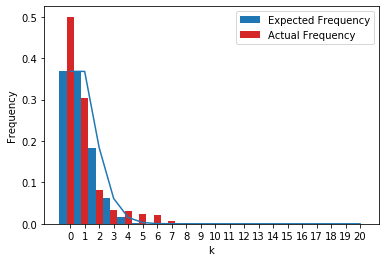
\includegraphics[width=10cm]{images/champ-16-freq.png}
%     \centering
%     \caption{Observed and expected frequencies for $n = 16$ and $\lambda = 1$}
%     \label{fig:champ-16-freq}
% \end{figure}

\begin{figure}[h]
    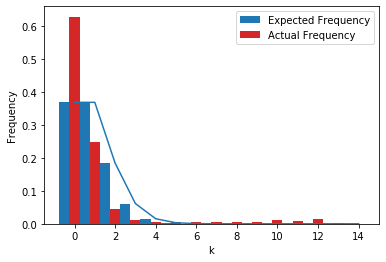
\includegraphics[width=0.75\textwidth]{images/champ-22-freq-2.png}
    \centering
    \caption{Observed and expected frequencies in $champ$ for $n = 22$ and $\lambda = 1$.}
    \label{fig:champ-22-freq}
\end{figure}

As it can be observed in Figure\ref{fig:champ-22-freq}, the amount of words of length $n$ that do not appear in the first $2^n$ symbols of $champ$ is much higher than the expected one for the sequence to be 1-supernormal. As we will observe later in the proof this is due to the fact that by the way that $champ$ is constructed.
This experiment as well a supernormality check for other famous normal sequences and a few pseudorandom number generators are available at ~\cite{Puterman}.

% One more interesting thing to do experimentaly is to check wether some pseudorandom number generators generate sequences that empiricaly appear to be supernormal. We analyzed what happened with sequences genereated with the Mersenne Twister PRNG which is the PRNG used by Python and with the cellular autmata Rule 30 which was used as the PRNG in Mathematica.

%% ...
\chapter{Supernormality is stronger than normality}
\section{Supernormality implies normality}

Recall that given an infinite  binary sequence $x$, and non-negative intergers $k$ and $n$,
$$A^\lambda_{k,n}(x) = \frac{\#\{w: |w| = n  , |x[1...\lfloor\lambda 2^n)\rfloor]|_w = k\}}{2^n}$$
The sequence $x$ is supernormal if for every positive real $\lambda$ and for every non-negative integer $k$,
$$\lim_{n\to\infty} A^\lambda_{k,n}(x) = \frac{e^{-\lambda}\lambda^k}{k!}$$ 



\begin{definition} 
  For the simplicity of the proof we define $a_k(\lambda)$ as the probability mass function of the Poisson distribution:
   $$a_k(\lambda) = \frac{e^{-\lambda}\lambda^k}{k!}$$
\end{definition}

We now observe a few useful facts:

\begin{fact}
    $$\sum_{k \geq 0} a_k(\lambda) = e^{-\lambda}\sum_{k \geq 0} \frac{\lambda^k}{k!} = e^{-\lambda}e^{\lambda} = 1$$
\end{fact}

\begin{fact}
    $$\sum_{k \geq 0} ka_k(\lambda) = e^{-\lambda}\sum_{k \geq 1} \frac{\lambda^k}{(k-1)!} = \lambda e^{-\lambda} \sum_{k \geq 0} \frac{\lambda^k}{k!}= \lambda$$
\end{fact}





\begin{fact}
    $$\sum_{k \geq 0} A^{\lambda}_{k,n}(x) = 1$$
\end{fact}

\begin{fact}
    $$A^{\lambda}_{k,n}(x) = 0 \textrm{ if } k > \lambda2^n$$
\end{fact}


Let's also recall that a sequence $x$ is normal if  for every binary word $w$,
\[
\lim_{n\to\infty} \frac{|x[1..n]|_w}{n}= 2^{-|w|}.
\]

Assume  $x$ is supernormal.
Fix a positive $\epsilon$.
Let $k_0$ be such that 
$$\frac{1}{\lambda} \sum_{k > k_0} ka_k(\lambda) < \frac{\epsilon}{2}$$

Let $n_0$ be  such that  for all 
$ i,n$ such that $  0 \leq i \leq k_0 $, $n > n_0$ and 
  $$|A^\lambda_{i,n}(x) - a_i(\lambda)| \leq \frac{\epsilon\lambda}{2k_0^2}$$


 $$\sum_{k=0}^{k_0} ka_k(\lambda) = \lambda - \sum_{k> k_0} ka_k(\lambda) \geq \lambda\Big(1 - \frac{\epsilon}{2}\Big)$$


We fix $\lambda$ equal to 1 for the simplicity of the proof, nonetheless the result is analogous with any value.
Consider the positions from $1$ to $ 2^n $ in $x$. 
We say that a position is \textit{blamed} if the word of length $n$ starting at that position 
occurs more than $k_0$ times in 
 $x[1..(2^n)]$. 

 The number of blamed positions 
 between  $1$ and $2^n$ is:

\begin{align*}
   2^n -  \sum_{k=0}^{k_0} kA^{1}_{k,n}(x) 2^n 
     &\leq 2^n - 2^n\Big(\sum_{k=0}^{k_0} k a_k(1) - \frac{\epsilon}{2k^2_0}\Big) \\
    &\leq 2^n -  \Big(2^n \sum_{k=0}^{k_0} ka_{k}(1)\Big) + \frac{2^n\epsilon}{2}\\
    &\leq 2^n - \Big(2^n \big(1-\frac{\epsilon}{2}\big)\Big) + \frac{2^n\epsilon }{2} \\
    &\leq 2^n\epsilon.
\end{align*}

We cover the positions from $1 $ to $2^n$ with consecutive
 non-overlapping blocks of length~$n$ such that 
no block starts at a blamed  position. 
This means that a block may contain blamed positions as long as they are not the first one. 
In the following example, the symbol $\times$ represents a blamed position:
 
$$\overbracket{\raisebox{6.4pt}{\qquad}}^{n} \overbracket{\raisebox{6.4pt}{\qquad}}^{n}\times\times\overbracket{\;\quad \times}^{n} \times \overbracket{\raisebox{6.4pt}{\qquad}}^{n} \overbracket{\raisebox{6.4pt}{\qquad}}^{n} \times \overbracket{\;\; \times \times}^{n} \times\times\times \overbracket{\raisebox{6.4pt}{\qquad}}^{n}$$


\begin{definition}
  Let $Bad(n, w, \epsilon)$ be the set of binary words of length $n$ where the word $w$ differs from the expected frequency by normality
 more than $n \epsilon$. Thus,
  $$Bad(n, w, \epsilon)=\Big{\{}v\in \{0,1\}^n: \Big{|} |v|_w - n 2^{-|w|} \Big{|} \geq \epsilon n \Big{\} }$$
\end{definition}


The cardinality of the set $Bad(n, w, \epsilon)$ is less than $2^{n+1} e^{-\epsilon^2 n/(6|w|)}$.
 This follows from  is a classical result from probability theory called Bernstein’s inequality (see for example \cite[Lemma 2.2.9]{VW}.   A detailed proof can be read from \cite[Lemma 7.3.5]{BC2018}. Therefore, the cardinality of the  \textit{bad} words of a given length $n$ decreases exponentially in~$n$.

Supernormality determines that  some blocks of length $n$
do not occur in $x[1\dots  2^n]$, and different blocks may 
have different number of occurrences.
%The idea now is to check that for a given word $w$ the blocks of length $n$ mantain the right frequencies.
We now fix $ n, \epsilon$ and $w$ and give an upper bound of  the number of occurrences of $w$ in 
$x[1 .. 2^n]$. To do so we consider the following:
\begin{enumerate}
\item Each blamed position can allocate at most one occurrence of $w$.
\item Each block in $Bad(n, w, \epsilon)$ can occur in $x[1.. 2^n]$
 at most $k_0$ times.
\item Each block in $Bad(n, w, \epsilon)$ has at most $n-|w|+1$ occurrences of $w$.
\item The sequence $x[1..  2^n]$ can be splitted in at most $ 2^n/n$ consecutive blocks
of length~$n$.  
\item Each block  of length $n$ that starts at a position that is not blamed,  and it is not a bad block
 contains at most $n 2^{-|w|} + \epsilon n $ occurrences of $w$.
\item In between two consecutive blocks of length $n$ there are at most $|w|-1$ occurrences of $w$.
\end{enumerate}
Thus,
\begin{align*}
|x[1.. 2^n]|_w \leq &
 \#\text{blamed positions} +
\\& k_0 \#(\text{bad blocks}) (n-|w|+1)+
\\& \#(\text{not bad blocks starting at non-blamed positions}) (n 2^{-|w|} + \epsilon n)+
\\&  \#(\text{in between blocks})  (|w|-1)
\\
\leq& 2^n \epsilon + 
\\& 2^{n+1} e^{-\epsilon^2 n/(6|w|)} (n-|w|+1)+
\\&  ( 2^n /n) (n 2^{-|w|} + \epsilon n)+
\\&  ( 2^n/n) (|w|-1)
\end{align*}
Hence, 
% \begin{align*}
% \frac{|x[1..  2^n]|_w }{ 2^n}&\leq 
%  \frac{n}{ 2^{n}} \epsilon+   \epsilon+
% 2 e^{-\epsilon^2 n/(6|w|)}  (n-|w|+1)+\frac{ \epsilon}{2^{n}}+
% +  \frac{1}{2^{|w|}} + (|w|-1)/n
% \end{align*}

\begin{align*}
  \frac{|x[1..  2^n]|_w }{ 2^n}&\leq \epsilon + 2 e^{-\epsilon^2 n/(6|w|)}  (n-|w|+1) + \frac{1}{2^{|w|}} + \epsilon + (|w|-1)/n
  \end{align*}


This  inequality above holds for every  for every $\epsilon$. By taking limit superior when $n$ goes to infinity we obtain 
\begin{align*}
\limsup_{n\to \infty}\frac{|x[1.. 2^n]|_w }{ 2^n} \leq {2^{-|w|}}
\end{align*}


To show that $x$ is normal it remains to see that the wanted 
limit holds when we count occurrences of any given word at initial segments of $x$ of arbitrary length:
\begin{align*}
\lim_{n\to \infty}\frac{|x[1.. n]|_w }{ n}= {2^{-|w|}}
\end{align*}

To get the wanted result we apply the  Hot Spot lemma, originally by Piatetski-Shapiro  and reconsidered 
later by Borwein and Bailey \cite{hotspot}  who gave it this name. For  the history and references see~\cite[Theorem 7.4.1]{BC2018}.
The Hot Spot lemma says that a binary sequence $x$ is normal if and only if there is a constant $C$ 
such that for infinitely many lengths $\ell$ and for every w in~$\{0,1\}^\ell$,
    $$\limsup_{N\to \infty}  \frac{|x[1.. N]|_w }{N} \leq C \frac{1}{2^{|w|}}$$
 We now determine that the constant $C$ exists and it is equal to $2$.
Fix $N$ and let $n$ be such that $2^{n-1}\leq N<2^{n}$. 
Then,
\begin{align*}
\frac{{|x[1.. N]|_w }}{N}\leq \frac{{|x[1.. 2^{n}]|_w }}{2^{n-1}}.
\end{align*}
Then, using the bounds obtained above,
\begin{align*}
\limsup_{N\to \infty}  \frac{|x[1.. N]|_w }{N} 
&\leq \limsup_{n\to \infty}\frac{{|x[1.. 2^{n}]|_w }}{2^{n-1}}\\
%&\leq \limsup_{n\to \infty}\frac{{|x[1.. 2^{n}]|_w }}{2^{n-1}}\\
&\leq 2\frac{1}{2^{|w|}}.
\end{align*}
Thus the constant $C$ is equal to $2$.
We conclude that $x$ is normal to base $2$.
\pagebreak

\section{Normality does not imply supernormality}
We aim to prove that normality does not imply supernormality. 
For this we prove that the Champernowne sequence, proved to be normal in~\cite{champern}, 
fails to be supernormal. For this we show that  it is not 1-supernormal.
Our strategy is similar to that used by Pirsic and Stockinger in ~\cite{PS2019}  where they proved that when $x$ is 
the Champernowne 
sequence then $(2^n x \mod 1)_{n\geq 1}$ fails the Poissonian pair correlation.
With a similar strategy  Becher, Carton and Mollo Cunningham ~\cite{BCC2019}
 proved that when $x$ is a sequence of nested perfect necklaces, then $(2^n x \mod 1)_{n\geq 1}$ fails the Poissonian pair correlation.

Let $X(n)$ be the concatenation of all words of length $n$ over the alphabet with two symbols $A=\{0,1\}$ in lexicographic order.  It is clear that $X(n)$ has length $n2^n$. Then, for example:
$$X(2) = 00 \: 01 \: 10 \: 11$$
Note that spaces were added for reading convenience.

Let $champ$
% the Champernowne sequence
 be the concatenation of $X(n)$ for $n = 1,2,\dots$
 Then the first symbols of the $champ$
% Champernowne 
sequence are:
$$champ = 0 \: 1 \: 00 \: 01 \: 10 \: 11 \: 000 \: 001 \: 010 \: 011 \: 100 \: 101 \: 110 \: 111 \: 0000 \: 0001 \: \dots$$

By the definition of $\lambda$-supernormality, if we take $\lambda = 1$, then we need to prove that there is a non-negative integer $k$ such that
%$$\lim_{n\to\infty} A_{k,n}(1) = a_k(1)$$  % aqui faltaba  negar  la igualdad
$$\lim_{n\to\infty} \frac{\#\{w: |w| = n  , |x[1...2^n]|_w = k\}}{2^n} \neq \frac{e^{-1}}{k!}$$

\bigskip

%First, let's see that given $d$, we define $k = 2^d$, 
In the sequel we use the following notation. Given  a positive integer $d$ we write $k$ to denote $2^d$.
Notice that if  $n \geq d + k + 1$ then $champ[1.. 2^n]$ contains the whole block $X(k)$.% covered in the first $2^n$ symbols of Champernowne.


\begin{fact}
For every $n$ greater than or equal to $2$  $\sum_{i=1}^n i2^i < 2^{n + \log(n) + 1}$.
\end{fact}

\begin{fact} \label{p2}
%    $X(k)$ accounts for half of the total amount of symbols in the first $2^{d+k+1}$ symbols of Chamernowne.
The sequence $X(k)$ occurs in $champ[1.. 2^{d+k+1}]$ and  the length of $X(k)$ is more than $2^{d+k}$.
\end{fact}
\begin{proof}
  $2^{d+k+1} = 2^{d+k}2$ and $X(k)$ has length $k2^k = 2^d2^k = 2^{d+k}$ 
\end{proof}

We prove that $champ$ is not supernormal by showing that the frequency of words
 of length $k+d+1$ that do not occur in the first $2^{k+d+1}$ symbols of the champ
 sequence is higher than the expected frequency if it were supernormal.
To accomplish this, we exhaustively count how many different words of length $2^{k+d+1}$ 
are there within $X(k)$ and give an upper bound for the amount of different words that can 
appear in the first $2^{k+d+1}$ symbols of the $champ$ sequence.

Now, let's see  the words of length $k + d + 1$ that occur in $X(k)$. % look like. 
%There are four different cases that can happen of how a word $x$ is formed with elements from $X(k)$. 
In the following analysis, $u, v$ and $w$ are consecutive words of length $k$ in $X(k)$.
If a  word $x$  of length $k + d + 1$  occurs in $X(k)$ it must be in one of these five cases, which are mutually exclusive:

\begin{itemize}
  \item \underline{Case 1:} 
  $$x = u_1 u_2 \dots u_k \quad v_1 v_2 \dots v_{d} v_{d + 1}$$
    Thus, $x$ occurs at a position $p\equiv k \mod 1$ 
   % modulo 1 for a given word $u$ of length $k$ in $X(k)$ plus the remaining $d + 1$ symbols which are taken from the next word.
    And $x$ is the concatenation of a word $u$ of length $k$ with $d+1$ symbols of the next word in the lexicographic order.

  \item \underline{Case 2:} 
  $$ x = u_{k-d-1} \dots u_k \quad v_1 v_2 \dots v_k$$
  Thus, $x$ is  the suffix of length $d + 1$ of a word of length $k$  concatenated with  the next word of length $k$
%word of length $k + d + 1$ is formed from the last $d + 1$ symbols of a word and the whole $k$ symbols of the next word.

  \item \underline{Case 3:} 
  $$x = u_{n+1} u_{n+2} \dots u_k \quad  v_1 v_2 \dots v_{d+n+1} $$
with $n \in \{1,2,\dots ,k - d - 2\}$.

Thus, $x$ is the concatenation of a proper suffix of a word of length $k$ and a proper prefix of the next word of length $k$ .
 %but  is the case where the $k + d + 1$ symbols are taken from two words of length $k$ and none of the words is complete.

  
  \item \underline{Case 4:} 
  $$ x = u_{k-d-1+n} u_{k-d+n} \dots u_k \quad v_1 v_2 \dots v_k \quad w_1 w_2 \dots w_{d+1-n}$$
  with $n \in \{1, 2, \dots , d\}$
  %Which is the case where the word of length $k + d + 1$ is formed by a full word, and the extra $d + 1$ 
% symbols are taken from both the end of the previous word and the beginning of the next one.
Thus, $x$ consist of a suffix of a word of length $k$ followed by the next  word of length $k$,
 followed by a prefix of  the next  word of length $k$.

  \item \underline{Case 5:} 
  
Consider that    $x$ occurs at the end of $X(k)$ or near the end of   $X(k)$ as follows. Either there is no complete word of length $k$ after $x$, 
or, if there are not two words of length $k$ after it. Notice that this case is excluded in  the previous cases.

%In the previous cases we considered every word $u$ such that there is a word $v$ and in case 4 two words 
%$v$ and $w$ that come after $u$ in $X(k)$. This is not true for the last two words of $X(k)$ so we consider them a different case.
  \end{itemize}



\subsection{Case Analysis}


%\begin{definition}
    The function  $next(w):A^n \rightarrow A^n $ is defined as follows. If $w$ is a row of $n$ many $1$s then  $next(w)$ is a row of $n$ many $0$s.
%Ibe $|w|$ times 0 if $w$ only consists of $1s$ and the word that comes after $w$ in lexicographic order in any other case.
Else, $next(w)$ is the word  after $w$ in lexicographic order.
%\end{definition}

\subsubsection{Case 1}
$$x = u_1 u_2 \dots u_k \quad v_1 v_2 \dots v_{d} v_{d + 1}$$

% \note{Redaccion}
This case accounts for the aligned occurrence of a given word $u$ of length $k$ in $X(k)$. The remaining $d + 1$ symbols are taken from the next word $v$.
As an example, some of the words of length $k + d + 1$ formed from $X(k)$ taking $k = 8, d = 3$ are shown between brackets:

$$( 00000000 \qquad 0000 ) \; 0001$$
$$( 00000001 \qquad 0000 ) \; 0010$$
$$( 00000010 \qquad 0000 ) \; 0011$$
$$\vdots$$
$$( 00001110 \qquad 0000 ) \; 1111$$
$$( 00001111 \qquad 0001 ) \; 0000$$
$$( 00010000 \qquad 0001 ) \; 0001$$
$$\vdots$$
$$( 11111110 \qquad 1111 ) \; 1111$$

We make two observations. The first one is that as the words of length $k + d + 1$ are formed by a full word of length $k$ followed by the first $d + 1$ symbols from the next word, in almost every case the first $d + 1$ symbols are equal to the last $d + 1$.
The only way for this not to happen, is when the last $k - d - 1$ symbols from the first word $u$ are all $1s$, which means that the next word in lexicographic order $v$ consists of $next(v_1 v_2 \dots v_{d + 1})$ concatenated with $next(v_{d + 2} v_{d + 3} \dots v_{k})$.

The second important thing to notice is that as $X(k)$ is the concatenation of all words of length $k$, 
all words of length $k$ occur one time in an aligned position modulo $k$. This means that $u$ will be every possible word of length $k$ once (except the last one in lexicographic order).
% \note{Esto esta mal redactado}

These two observations determine two possible schemes for what a word $x$ of case 1 may look like:

$$\underbrace{\quad A \quad }_{d +1} \qquad \underbrace{\quad B \quad }_{k - d - 1}  \qquad A$$


$$\underbrace{\quad A \quad }_{d +1} \qquad \underbrace{ 11 \dots 1  }_{k - d - 1}  \qquad next(A) $$
For the first scheme we have:
$$2^{d + 1}  (2^{k - d - 1} - 1) =  2^k - \frac{1}{2\cdot2^{d} }$$
%$$ 2\cdot2^{d}  (\frac{2^k}{2\cdot2^d} - 1)$$
%$$ 2^k - \frac{1}{2\cdot2^{d} }$$
%$ 2^k - \frac{1}{2\cdot2^{d} }$ 
different words.

For the second scheme we subtract one to the cases due to the fact that the last word of length $k$ in $X(k)$ has its continuation outside $X(k)$:
$$2^{d + 1}   - 1$$
%$$2\cdot 2^d - 1$$
%$ 2\cdot 2^d - 1 $ 
different words.
\\

Counting the whole case together we have $  2^k - \frac{1}{2\cdot2^{d} } + 2\cdot 2^d - 1$ which is less than $2^k -  2\cdot 2^d$ different words.

\subsubsection{Case 2}
$$ x = u_{k-d-1} \dots u_k \quad v_1 v_2 \dots v_k$$

% \note{redaccion}
This case accounts for the aligned occurence
of a given word $v$ of length $k$ in $X(k)$ plus the remaining $d + 1$ symbols which are taken from the previous word. In this case every single word of length $k$ will take the place of $v$, except for the first one in lexicographic order.
As an example, some of the words of length $k + d + 1$ formed from $X(k)$ taking $k = 8, d = 3$ are shown between brackets:

$$0000 \; (0000 \qquad 00000001)$$
$$0000 \; ( \; 0001 \qquad 00000010)$$
$$\vdots$$
$$0000 \; (1111 \qquad 10000000)$$
$$1000 \; (0000 \qquad 10000001)$$
$$\vdots$$
$$1111 \; (1110 \qquad 11111111)$$

As in the previous case, as $X(k)$ is the concatenation of all words of length $k$, all words of length $k$ occur one time in an aligned position modulo $k$. This means that the last $k$ symbols of $x$ take every possible configuration.
The other important thing to notice is that as the first $d + 1$ symbols of $x$ come from the word $u$ which occupies exactly before $v$ in lexicographic order, then: 
$$next(u_{k-d-1} u_{k-d} \dots u_k) = u_{v-d-1} v_{k-d} \dots v_k$$

This determines only one possible scheme for what a word $x$ of case 2 may look like:

$$\underbrace{\quad A \quad }_{d +1} \qquad \underbrace{\quad B \quad }_{k - d - 1}  \qquad next(A)$$
This scheme gives us the following amount of different words that may occur:
$$(2^{d + 1} 2^{k-d})-1=  2 \cdot 2^k - 1$$
%$$ 2\cdot 2^d  (\frac{2^k}{2^d}) - 1$$
%$$ 2 \cdot 2^k - 1$$
%$ 2 \cdot 2^k - 1 $ 
different words which is less than $2 \cdot 2^k$ different words.

\subsubsection{Case 3}
$$x = u_{n+1} u_{n+2} \dots u_k \quad  v_1 v_2 \dots v_{d+n+1} $$
with $n \in \{1,2,\dots ,k - d - 2\}$.
\\

This case accounts for when the $k + d + 1$ symbols are taken from two words of length~$k$ and none of the words is complete.
As an example, some of the words of length $k + d + 1$ formed from $X(k)$ taking $k = 8, d = 3$ are shown between brackets
Some extra spaces are added within $u$ and $v$ to make clear the scheme explained later.
Taking $n = 1$.


$$0\; (0000\; 000 \qquad 0 \;0000 ) \;001$$
$$0\; (0000 \;001 \qquad 0 \;0000 ) \;010$$
$$\vdots$$
$$0\; (0001 \;110 \qquad 0 \;0001 ) \;111$$
$$0\; (0001 \;111 \qquad 0 \;0010 ) \;000$$
$$0\; (0010 \;000 \qquad 0 \;0010 ) \;001$$
$$\vdots$$
$$1\; (1111 \;101 \qquad 1 \;1111 ) \;110$$
$$0\; (1111 \;110 \qquad 1 \;1111 ) \;111$$

Taking $n = k - d - 2 = 3$

$$000\; (0000\; 0 \qquad 000 \;0000 ) \;1$$
$$000\; (0000\; 1 \qquad 000 \;0001 ) \;0$$
$$000\; (0001\; 0 \qquad 000 \;0001 ) \;1$$
$$000\; (0001\; 1 \qquad 000 \;0010 ) \;0$$
$$\vdots$$
$$111\; (1110\; 1 \qquad 111 \;1111 ) \;0$$
$$111\; (1111\; 0 \qquad 111 \;1111 ) \;1$$

In this case, it also happens that as $X(k)$ is the concatenation of all words of length $k$, for each value of $n$, all words of length $k$ take the $u$ position once, except the last of the words of length $k$ in $X(k)$.

It is important to notice that for a given value of $n$, the first $n$ symbols of $u$ are not be considered to form $x$. This means that it can be interpreted that the symbols from  $u$ that are considered are, the first $d + 1$ symbols after $n$ which are called $A$ and the remaining $k - d - 1 - n$ symbols which are be called $B$.

Now, if we divide the $n + d + 1$ symbols that are used from $v$ to form $x$ into the first $n$ symbols which are called $C$ and the remaining $d + 1$ symbols, it is possible to see that these $d + 1$ symbols are always equal to the symbols from $A$ except for the case where $B$ = $11\dots1$ as they account for the same indexes of $u$ and $v$ and $v$ comes immediately after $u$ in lexicographic order. 


These leave two possible schemes for what a word x of case 3 may look like:

$$\underbrace{\quad A \quad }_{d +1} \qquad \underbrace{\quad B \quad }_{k - d - 1 - n}  \qquad \underbrace{\quad C \quad }_{n} \qquad A$$

$$\underbrace{\quad A \quad }_{d +1} \qquad \underbrace{\; 11\dots1 \; }_{k - d - 1 - n}  \qquad \underbrace{\quad C \quad }_{n} \qquad next(A)$$

Looking closely at the first scheme, it is possible to see, if we put together $B$ and $C$ which have length $k - d - 1 - n$ and $n$ respectively, that we have the following scheme:

$$\underbrace{\quad A \quad }_{d +1} \qquad \underbrace{\quad B \quad }_{k - d - 1}  \qquad A$$

which is exactly the same one as in case 1. This means that all the possible words that can be formed following this scheme don't yield any new words.
\\
The same thing happens with the second scheme when concatenating $11\dots1$ with $C$:

$$\underbrace{\quad A \quad }_{d +1} \qquad \underbrace{\; 11\dots1C \; }_{k - d - 1}  \qquad next(A)$$

Which is a particular case of case 2.

This means that for case 3 there are no words that appear that should be taken into account as new words.


\subsubsection{Case 4}
$$ x = u_{k-d-1+n} u_{k-d+n} \dots u_k \quad v_1 v_2 \dots v_k \quad w_1 w_2 \dots w_{d+1-n}$$
with $n \in \{1, 2, \dots , d\}$

This case accounts for when the $k + d + 1$ symbols are taken from three words of length~$k$. The $k$ symbols of $v$ are used and the remaining $d + 1$ symbols are taken from both the previous and the following words $u$ and $w$.
As an example, some of the words of length $k + d + 1$ formed from $X(k)$ taking $k = 8, d = 3$ are shown between brackets
Some extra spaces are added within $u$ and $v$ to make clear the scheme that is explained later.

Taking $n = 1$.
$$0000000\; (0 \qquad 000 \; 0000 \; 1 \qquad 000) \: 00010$$
$$0000000\; (1 \qquad 000 \; 0001 \; 0 \qquad 000) \: 00011$$
$$\vdots$$
$$0011111\; (0 \qquad 001 \; 1111 \; 1 \qquad 001) \: 10000$$
$$0011111\; (1 \qquad 010 \; 0000 \; 0 \qquad 010) \: 00001$$
$$\vdots$$
$$1111110\; (1 \qquad 111 \; 1111 \; 0 \qquad 111) \: 11111$$

Taking $n = 2$.
$$000000\; (00 \qquad 00 \; 0000 \; 01 \qquad 00) \: 000010$$
$$000000\; (01 \qquad 00 \; 0000 \; 10 \qquad 00) \: 000011$$
$$\vdots$$
$$001111\; (01 \qquad 00 \; 1111 \; 10 \qquad 00) \: 111111$$
$$001111\; (10 \qquad 00 \; 1111 \; 11 \qquad 01) \: 000000$$
$$001111\; (11 \qquad 01 \; 0000 \; 00 \qquad 01) \: 000001$$
$$\vdots$$
$$111111\; (01 \qquad 11 \; 1111 \; 10 \qquad 11) \: 111111$$

In this case, it also happens that as $X(k)$ is the concatenation of all words of length $k$, for each value of $n$, 
all words of length $k$ take the $u$ position once, except the last of the words of length $k$ in $X(k)$.

We call $A$ the first $n$ symbols of $x$ which are taken from the end of $v$. The following $d + 1 - n$ symbols which are the first of $v$ are called $B$ and it happens that unless the remaining symbols of $v$ are all $1s$, 
they are the same as the last $d + 1 - n$ of $x$ because these symbols are the first $d + 1 - n$ from $w$.
Now, we consider the remaining $k - d - 1 + n$ symbols from $v$ as two blocks, one block $C$ of length $k - d - 1$ and the remaining $n$ symbols which are exctly $next(A)$ as $v$ is the next word in lexicographic order after $u$.
This yields the following two schemes:

$$\underbrace{\quad A \quad }_{n} \qquad \underbrace{\quad B \quad }_{d + 1 - n}  \qquad \underbrace{\quad C \quad }_{k-d+1} \qquad next(A) \qquad B$$

$$\underbrace{\quad 11\dots10 \quad }_{n} \qquad \underbrace{\quad B \quad }_{d + 1 - n}  \qquad \underbrace{\; 11\dots1 \; }_{k-d+1} \qquad next(A) \qquad next(B)$$

For the first scheme we have:

$$\sum_{n=1}^{d}(2^n - 1) (2^{d + 1 - n}) (2^{k - d - 1})$$
$$\sum_{n=1}^{d}(2^n - 1) (\frac{2 \cdot 2^d}{2^n})     (\frac{2^k}{2 \cdot 2^d})$$
$$ 2^k \sum_{n=1}^{d} \frac{2^n - 1}{2^n} $$

% Here we would need to substract the cases for when $v$ is the last word of $X(k)$, however as we are giving an upper bound for the words that appear in Champernowne, the result still holds taking this number.

For the second scheme we have:

$$ \sum_{n=1}^{d} 2^{d + 1 - n}$$
$$ \sum_{n=1}^{d} 2 \frac{2^d}{2^{- n}}$$
$$ 2 \cdot 2^d \sum_{n=1}^{d} 2^{- n}$$

When putting them both together we get:

$$  2^k \sum_{n=1}^{d} \frac{2^n - 1}{2^n}  + 2 \cdot 2^d \sum_{n=1}^{d} 2^{- n} < d2^k + 2 \cdot 2^d$$

\subsubsection{Case 5}

We consider the last two words of $X(k)$ as special cases. The last word of $X(k)$ does not apply to any of the cases since there are no words $v$ and $w$ inside $X(k)$ to consider the cases. Something similar occurs with the word previous to the last one and case 4. 
While it is true that we do know which words come immediately after  $X(k)$, which are the first words of size $d+k+2$ in lexicographic order, as we are giving an upper bound, it is valid to consider all of these as different words to all of the ones considered in the previous cases.
By doing this, we would have to consider $d+k+1$ new words for the last word and $d$ words for the previous one. So this yields $2d+k+1$ words to consider.


\subsection{A bound for the number of words occurring in $champ$}%Bounding words that appear in Champernowne}

% \note{en todos lados hay que poner $champ$ en vez de Champernowne}
If the $champ$ %Champernowne
 sequence were supernormal then the expected frequency of words that appear at least one time in the first $2^n$ symbols would satisfy:
$$\lim_{n\to\infty} \frac{\#\{w: |w| = n  , |champ[1...2^n]|_w > 0\}}{2^n}  = 1 - e^{-1}$$


Now, by Fact \ref{p2} we know that $X(k)$ accounts for half of the words of the first $2^{d+k+1}$ symbols of $champ$. 
If we analyze what happens with words of length $d+k+1$ using the bounds we have for the occurrences of different words within $X(k)$ and we assume that the remaining $2^{d+k} + d + k - 1$  symbols are all different, then


\begin{align*}
&\limsup_{d\to\infty} \frac{\#\{w : |w| = d+k+1, |champ[1 \dots 2^{d+k+1}]|_w > 0 \}}{2^{d+k+1}} <\\
&\limsup_{d\to\infty} \frac{ \textrm{Case 1} + \textrm{Case 2}+ \textrm{Case 4} + \textrm{Case 5} + \textrm{other half}}{2^{d+k+1}} =\\
&\limsup_{d\to\infty} \frac{(2^k - 2\cdot 2^d) + (2 \cdot 2^k)+ (d2^k + 2 \cdot 2^d) + (2d+k+1) + (2^{d+k}) }{2^{d+k+1}} =\\
&\limsup_{d\to\infty} \frac{(2^k - 2k) + (2 \cdot 2^k)+ (d2^k + k) + (2d+2k+1) + (k2^{k})}{2k2^{k}} =\\
&\limsup_{d\to\infty} \frac{3\cdot2^k + d2^k  + 2d+k+1}{2k2^{k}} + \frac{1}{2} =\\
&\limsup_{d\to\infty} \frac{3}{2k} + \frac{d}{2k} + \frac{d}{k2^{k}} + \frac{1}{2\cdot2^{k}} + \frac{1}{2k2^{k}} + \frac{1}{2} = \frac{1}{2} \\
&< 1 - e^{-1}
\end{align*}

Finally, if in the original sequence we consider that the $n$'s such that $n = d + 2^d + 1$ are a subsequence of $n=1,2,\dots$ then we can say that if
$$\lim_{n\to\infty} \frac{\#\{w: |w| = n  , |champ[1...2^n]|_w > 0\}}{2^n}$$
exists, then it is not $1 - e^{-1}$.
This implies that Champernowne is not 1-supernormal which means it is not supernormal.

\begin{corollary}
If $x$ is a normal number it is not implied that $x$ is supernormal.
\end{corollary}


% \chapter{Conclusions and Further Work}

%%%% BIBLIOGRAFIA
%\chapter{Bibliography}
\backmatter
% \note{Emprolijar la bibliografia. O bien todos van con nombre y apellido, o bien todos con inicila y apellido}
\bibliographystyle{acm}
\bibliography{tesis}



\end{document}
